\label{chap:basics}
This is basics.
	\section{Formal power model}
	There are two central concepts for memory power optimization using the memory partitioning method.
	One concept is the allocation $ \alpha $ which is a set of memory instances of certain memory types. Memory
	types are defined by the physical characteristic parameters such instance size, area, read current
	and so on.The other concept is the binding $ \beta $ of application code and data fragments to the 
	selected memory instances. The code and data fragments of an application are refereed as profiles
	of this application. And each application is represented by a set of profiles. Every profile is
	characterized by some user-defined parameters. Because all the code and data should be stored in
	the memories, each profile should be bound to exactly one memory instance \cite{Strobel2016}. 
	A configuration for the memory system is defined as the combination of an allocation of memory 
	instances and the corresponding binding for the application profiles. The goal of memory power 
	optimization is to find a configuration among all possible configurations such that the overall 
	power consumed by all selected memory instances is the lowest under certain predefined constraints.
	Therefor, the memory power optimization can be achieved by the facts 
	that smaller memory instances consume less power and the larger memory instances are 
	seldom accessed.
	\label{sec:power_model}
	
	\section{Heuristics}
	\label{sec:heuristics}
	There are a lot of existing heuristics. At the early time of heuristics usage, the algorithms are applied to solve one
	particular optimization problem. These problem-dependent heuristics cannot be adapted to other optimization processes.
	To improve the portability of heuristics, some algorithms are invented as parameterized interface that can be widely
	deployed for a variety of optimization problems. Such problem-independent heuristics usually consist of a base framework
	with several parameters. Only the parameters are related to the optimization problems. When using one of those
	heuristics for different problem sets, the algorithm framework is common while the parameters should be set up according
	to the problem requirements. In the recent years, there is a new trend of heuristic which is called hyper-heuristic.
	The hyper-heuristics provide a high-level strategy to seek one or several low-level heuristics to generate a proper algorithm for solving an optimization problem. The hyper-heuristic is a cutting-edge technique and it is beyond the knowledge of this work. For the memory power optimization, the problem-independent heuristics are the mainly focused
	because of its extensive usage.
	
	There are a variety ways to classify the heuristics. One common classification is to differentiate the algorithms
	according to their searching mechanisms. To be simplified, the heuristics are divided as local search-based and
	non-local search-based in this work. The well known local search algorithm aims to seek for the optimal solution by
	iteratively moving to a better solution in the neighborhood. However, the local search is greedy and cannot guarantee providing the good enough solutions because it may trap in local optimums. The idea of local search-based heuristics
	is to avoid the local optimum trap through some criteria for solution selection and improve the result's quality.
	Heuristics of this kind output only one single optimal solution. Some classical local search-based heuristics are simulated annealing, tabu search, guided local search, etc. Unlike local search-based heuristics, the non-local search-based heuristics usually seek for a set of good enough solutions. By manipulating some defined solution characteristics, it can guide the searching process to the global optimums. Some typical non-local search-based heuristics are genetic algorithm, particle swarm optimization, ant colony optimization, etc.
	Normally, the frameworks of non-local search-based heuristics are more complicated than that of local search-based algorithms. And the expected result for memory power optimization is one optimal configuration not a set of
	configurations. Therefor, the local search-based heuristics are the main focuses in this work.
	In this section, the local search algorithm along with its local optimum trap is discussed first. Then, two typical
	local search-based heuristics, tabu search and simulated annealing, are represented. Lastly, the most promising algorithm 
	is proposed to the memory power optimization according to the comparison between these heuristics.
	
		\subsection{Local search algorithm}
		\label{subsec:local_search}
		Local search algorithm is one of the simplest heuristics. Given a optimization problem, it starts from an initial solution and searches in the current solution's neighborhood. If a better solution is found, the current solution is replaced by it. The searching process is repeated until there is no better solution in the current solution's neighborhood. Then it outputs the current solution as the algorithm result.
		Algorithm \ref{algo:local_search} shows the pseudo-code of local search process. There are four main steps in the algorithm. First step is finding a initial solution and set it as the current solution. The initial solution should be valid for the problem. In the second step, a neighboring solution is generated by certain mechanism. And the third step is to compare the neighboring solution with the current one through a object function. The object function is a method to indicate how good the solution is. The last step is the selection criterion for solution. Local search algorithm selects the better one between the current and neighboring solutions, which is a naive criterion.
		
		\setlength{\textfloatsep}{0.2cm}
\begin{algorithm2e}[htb]
	\KwIn{an optimization problem}
	\KwOut{an optimal solution}
	current solution = initial solution\;
	\While{not terminate}
	{
		generate a neighboring solution\;
		evaluate the neighboring solution\;
		\If{neighboring solution is better than current solution}
		{
			current solution = neighboring solution\;
		}
	}
	\Return current solution\;
	\caption{Local Search Algorithm}
	\label{algo:local_search}
\end{algorithm2e}
\setlength{\textfloatsep}{0.2cm}
		
		Though local search algorithm is simple, the solution it provides may be the local optimal one. This is the major problem of
		local search algorithm. Figure \ref{fig:local_optimum_local_search} illustrates this local optimum trap. Suppose the
		optimization problem is to find the solution with minimum cost, the local search algorithm starts with the initial solution $a$.
		The cost of neighboring solution $b$ is lower than cost of $a$, then $b$ becomes the current solution. The same searching process 
		is repeated until the current solution reaches $c$. There is no better solution in $c$'s neighborhood, thus the algorithm outputs solution $c$ and terminates. However, solution $c$ is only the local optimum and the global optimum is solution $e$ which
		is not in $c$'s neighborhood. In order to reach solution $e$, the algorithm has to move to solution $d$ whose cost is higher than
		$c$'s cost. And this violates the selection criterion of the algorithm. Another drawback of local search algorithm is that the result quality is dependent on the initial solution. If the algorithm starts with solution $d$, the output will be the global optimum $e$. These two disadvantages make local search algorithm an improper choice when global optimal solution is required for 
		the optimization problems.
		
			\begin{figure}[H]
				\begin{center}
					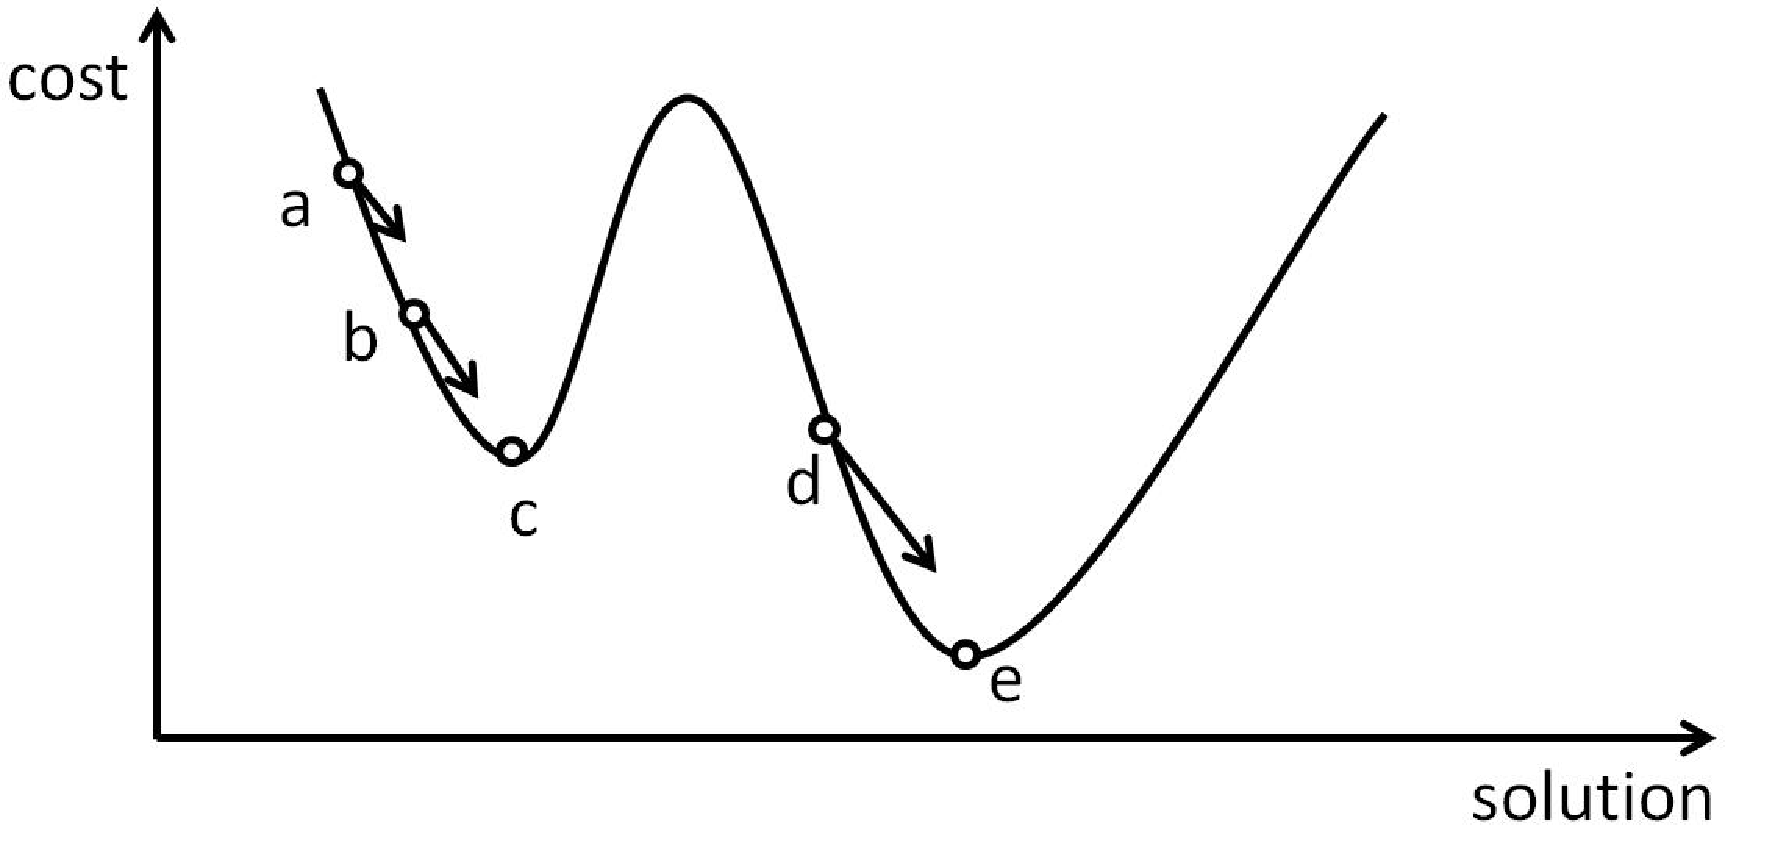
\includegraphics[width=0.7\textwidth]{local_optimum_local_search}
					\caption[Local Optimum Trap]{Local Optimum Trap}
					\label{fig:local_optimum_local_search}
				\end{center}
			\end{figure}
		
		\subsection{Tabu search algorithm}
		\label{subsec:tabu_search}
		One of the improvements to local search is the tabu search algorithm. It is based on local search but it avoids to stuck at the
		local optimal trap through a different selection strategy for solutions. As discussed in section \ref{subsec:local_search}, once
		the local search algorithm is trapped at a local optimal solution, it cannot move any further due to the naive solution criterion.
		To solve this problem, Fred Glover proposed the concepts of tabu list and the aspiration criterion in \cite{doi:10.1287/ijoc.1.3.190} and \cite{doi:10.1287/ijoc.2.1.4}.
		
		The key element of tabu search is the tabu list. It imitates the memory function of human brain to guide the searching process.
		It is used to record the tabu objects. The tabu objects can be defined as the solutions, solution movements or values of the 
		object function. Tabu list has a limited size which is one of the algorithm parameters. The improvement to local search algorithm
		is gained from the solution selection strategy that is usually called the tabu move. There are two rules in the tabu move. The
		first rule is to exclude the solutions recorded in the tabu list from a set of neighboring solutions. The second rule is to
		select the best in the rest of the neighboring solution set. The solution chosen by the tabu move is set as the current solution.
		Another concept of tabu search algorithm is the aspiration criterion. During the searching process, the best-so-far solution is
		kept recorded in the searching history. The aspiration criterion is to examine the neighboring solution set to find if there are solutions that are better than current best-so-far solution. If such solutions are found, then the best of them is selected and
		set as the current solution even if it is recorded in the tabu list. If no such solutions is found, the algorithm continues with
		the tabu move.
		
		\setlength{\textfloatsep}{0.2cm}
\begin{algorithm2e}[htb]
	\KwIn{an optimization problem, algorithm parameters}
	\KwOut{an optimal solution}
	set algorithm parameters\;
	current solution = initial solution\;
	best-so-far solution = initial solution\;
	set tabu list as empty\;
	\While{not terminate}
	{
		generate a set of neighboring solutions\;
		evaluate neighboring solutions\;
		\eIf{aspiration criterion satisfied}
		{
			execute aspiration criterion\;
			update current solution\;
			update tabu list\;
			update best-so-far solution\;
		}
		{
			execute tabu move\;
			update current solution\;
			update tabu list\;
		}
	}
	output current solution\;
	\caption{Tabu Search Algorithm}
	\label{algo:tabu_search}
\end{algorithm2e}
\setlength{\floatsep}{0.2cm}		
		
		Algorithm \ref{algo:tabu_search} is the pseudo-code of tabu search framework based on the Fred Glover's proposal in \cite{doi:10.1287/ijoc.1.3.190}. 
		At the beginning of the algorithm, it generates a valid initial solution and set it as the current solution and the best-so-for solution. The parameters are set up according to the algorithm inputs. And a tabu list is created as empty.
		After the initialization, the algorithm generates a set of neighboring solutions by some certain mechanism and evaluate it by an object function. After this step, there are two different branches.
		One branch is the execution of aspiration criterion. If the condition of the criterion is satisfied, the solution selected by the
		criterion is set as the current solution and the best-so-far solution. Also, the updated current solution is added to the tabu
		list. There are two cases for the tabu list updating. At the early stage of the algorithm, the list is not full. The solutions are added into the list sequentially. When there is no space for a new recorded solution, the oldest solution in the list is replaced by the new one.
		The other branch, tabu move, is executed when the condition of aspiration criterion is not satisfied. The current solution and the tabu list are updated with the solution chosen by the tabu move. And the best-so-far solution is not updated because there is no solutions better than it.
		The same searching process is repeated until the termination condition is satisfied and the algorithm outputs the current or the best-so-far solution as the optimization result. Some algorithm parameters are related to the termination condition. One simple
		method to terminate the algorithm is to set a fixed iteration number. Thus this fixed number is one parameter of the algorithm. However, this method cannot guarantee the solution quality. Another common termination mechanism is to count the appearance of the current solution. If the current solution dose not change for a max number iterations, the algorithm can terminate. Therefor,
		this max number is also one algorithm parameter.
		
		Figure \ref{fig:local_optimum_tabu} illustrates how the tabu search algorithm avoids the local optimum trap. The solid line represents the execution of the aspiration criterion and the dotted line is the tabu move.
		The same problem set in section \ref{subsec:local_search} is used. The tabu search algorithm starts from initial solution $a$ with an empty tabu list (assume the list size is large enough).
		After the neighboring solutions are generated, it finds solution $b$ satisfies the aspiration criterion. Then $b$ becomes the current
		solution and the best-so-far solution is updated to $b$ as well. Also, $b$ is added to the tabu list. Known from the figure, solution $b$ is
		a local optimum and there is no neighboring solution satisfies the aspiration criterion. Thus, the algorithm continues with the tabu move.
		During the tabu move, solution $b$ is excluded from the generated neighboring solution set because it is stored in the tabu list.
		And solution $c$ is found to be the best among the rests of the set. Thus, $c$ becomes the current solution and it is added to the tabu list.
		In the next iteration, solution $b$ and $d$ both are $c$'s neighboring solutions. However, $b$ is still in the tabu list and the aspiration
		criterion is not satisfied. Thus, the current solution $d$ is selected by the tabu move as it is the best among the rest of neighboring solutions.
		The same searching process is repeated until the algorithm reaches solution $e$ which is the global optimum.
		By selecting a worser solution in the tabu move, the tabu search algorithm can move to a new searching region and avoid the local optimum trap.
	
		%Tabu search problem, tabu size, too long computation time, too short loop searching, local optimal trap.
		%Dead lock, no aspiration criterion, neighboring solutions all tabued.
		%Dependent on the initial solution.
		\begin{figure}[H]
			\begin{center}
				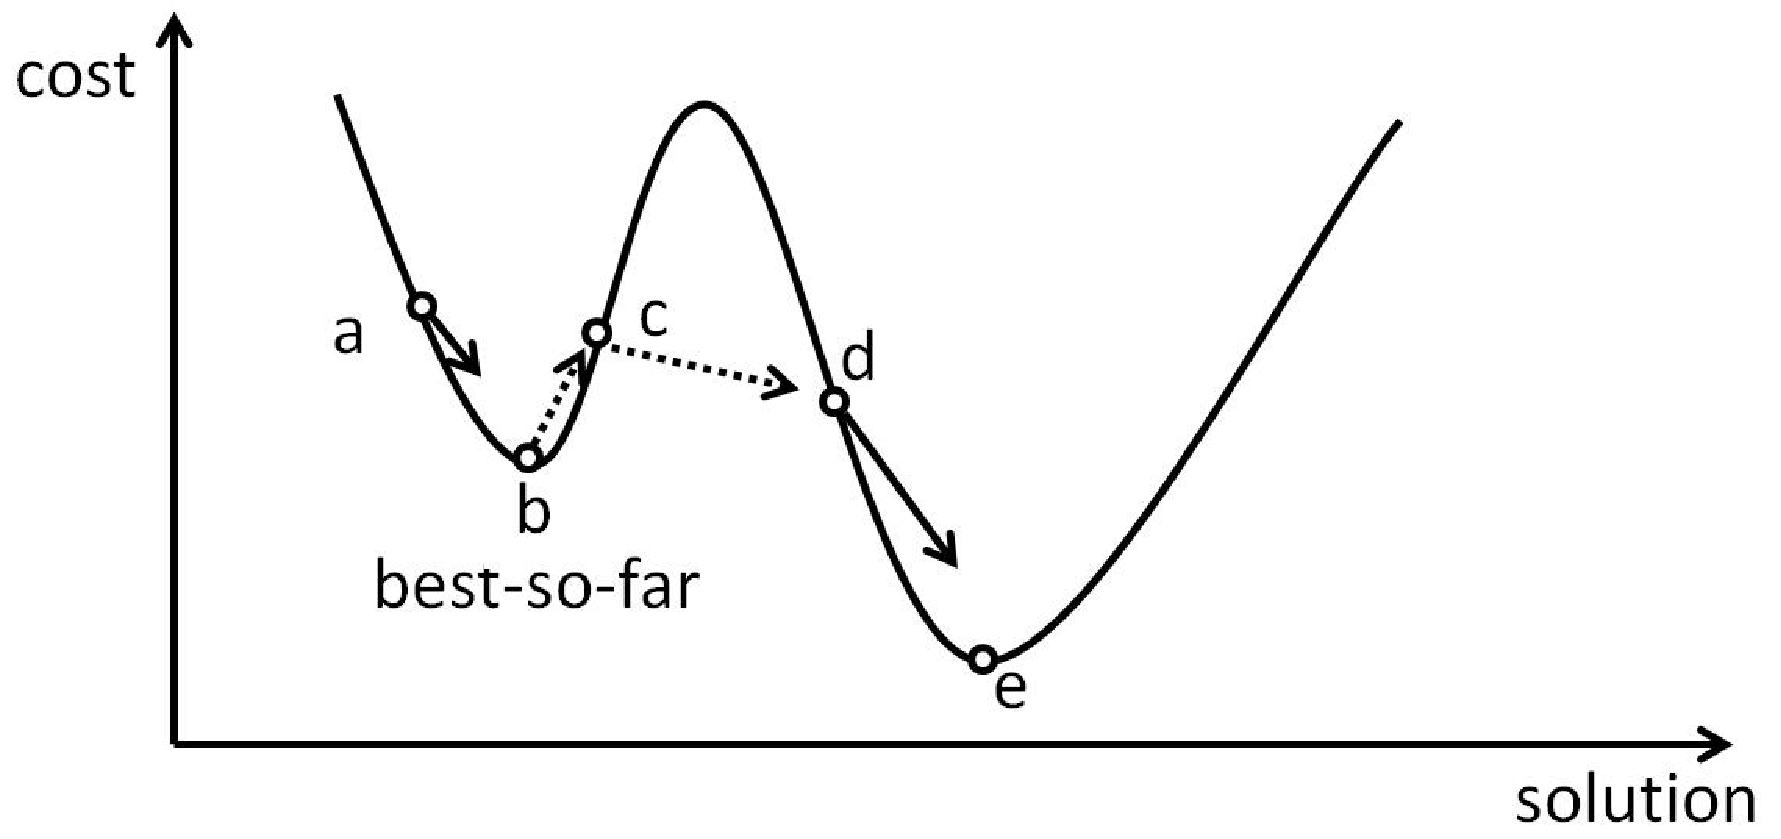
\includegraphics[width=0.7\textwidth]{local_optimum_tabu}
				\caption[Tabu Search's Avoidance to Local Optimum Trap]{Tabu Search's Avoidance to Local Optimum Trap}
				\label{fig:local_optimum_tabu}
			\end{center}
		\end{figure}
				
		
		
		
		
		
		
		
		
		
		
		
		
		
		